% Analítica Predictiva y Prescriptiva · TIC-60286 · Semana 4
% Juzgar modelos con dinero
% Compilar: pdflatex week-04.tex (dos veces)
%
% Plan de los 90 minutos
%   0–5    Dónde vamos y la encuesta de apertura (láminas 2–3)
%   5–20   El paper: Kleinberg et al. (2018), jueces y libertad provisional (láminas 4–8)
%  20–65   La aplicación: las consultoras A y B punto por punto, el dinero, las ventas, el giro (láminas 9–22)
%  65–70   Puente: el task 4 (lámina 23)
%  70–90   Cierre: la cacería del task 3 (lámina 24)
%
% Las cifras citadas están en datasets/aperturas/cifras_week04.txt (el sobre de la semana).
% Las figuras salen de week-04/input/_datos_y_figuras_week04.R (R base, la paleta del curso);
% juez_beneficio.pdf se copia de datasets/aperturas/figuras/.
% El giro de la lámina 21 (evaluar cuesta el triple, c = 36) no está en el sobre: lo imprime el
% mismo script al final (u = 0.5: A 782, B 600; u = 0.25: A 157, B -150; quiebre 0.864).
% ERROR SEMBRADO (lámina 9): el punto de venta 41 bajo la consultora B aparece como TN; es FP
% (B dijo riesgoso con 0.506 y el punto de venta siguió abierto). La sala debe encontrarlo.

\documentclass{beamer}
\input{../../_beamer/preambulo_app.tex}
\usepackage{colortbl}
\definecolor{grisclaro}{HTML}{F2F3F6}
\semana{4}{Juzgar modelos con dinero}

\begin{document}

%%=================================================
%% Primer slide
\begin{frame}
\titlepage
\end{frame}

%% ====================================================== 0. DÓNDE VAMOS (0–5)
\begin{frame}{Dónde vamos}
\begin{columns}[T]
\begin{column}{0.5\textwidth}
\textbf{La semana pasada:} el task 3, tres hallazgos con cifra sobre el estudio de aperturas, la columna prohibida y el acta del agente. Se discute hoy, en el cierre, contra el sobre.

\medskip
\textbf{Hoy, la pieza 4 del expediente:} el juicio de los modelos. Dos firmas de analítica, las consultoras A y B, ofrecen predicciones de cierre y de ventas. Dos tablas del líder, una recomendación (A, B o ninguna) y el supuesto que la voltea.
\end{column}
\begin{column}{0.5\textwidth}
\begin{block}{La sesión}
\begin{enumerate}
  \item El paper: jueces, libertad provisional y una predicción medida en crímenes y presos.
  \item Las consultoras A y B, punto por punto.
  \item El dinero: el costo de cada lista, el beneficio neto, la efectividad de quiebre.
  \item Las ventas: MAE y RMSE contra la regla del sector.
  \item El giro, y el task 4.
  \item Cierre: la cacería del task 3.
\end{enumerate}
\end{block}
\end{column}
\end{columns}
\end{frame}

\begin{frame}{Antes de empezar}
\parada{encuesta}{Dos consultoras ofrecen un modelo que predice si un local cerraría antes de tres años. En el lote de validación, A tiene \textbf{85.8\,\%} de exactitud y B \textbf{79.2\,\%}. ¿Cuál compras: A, B o ninguna?}
\pause
\medskip
Un dato antes de votar de nuevo: en ese lote cerró uno de cada cinco puntos de venta. ``Ningún punto de venta cierra'' acierta el \textbf{80.0\,\%} sin mirar un solo dato.
\end{frame}

\seccion{El paper: jueces, libertad provisional y una predicción}
%% ====================================================== 1. EL PAPER (5–20)
\begin{frame}{¿Puede un algoritmo mejorar las decisiones de un juez?}{Kleinberg, Lakkaraju, Leskovec, Ludwig y Mullainathan (2018), \emph{Quarterly Journal of Economics}}
\begin{columns}[T]
\begin{column}{0.5\textwidth}
\textbf{Qué investigaron.} Si un algoritmo que predice el riesgo de un acusado puede mejorar las decisiones de libertad provisional de los jueces: a quién dejar en libertad mientras llega el juicio y a quién mantener preso.

\medskip
\textbf{Por qué es una predicción.} La ley le pide al juez una sola cosa: estimar si el acusado se fugará o cometerá un delito si lo libera. No hay que decidir qué es justo; hay que predecir bien. Es una decisión con una predicción en el centro.
\end{column}
\begin{column}{0.5\textwidth}
\begin{block}{La trampa}
Un juez que acierta ``mucho'' no es necesariamente un buen juez: la mayoría de los acusados no se fuga, así que liberar a todos ya acierta en la mayoría de los casos. Suena conocido.
\end{block}
\end{column}
\end{columns}
\end{frame}

\begin{frame}{Qué datos y cómo}
\begin{columns}[T]
\begin{column}{0.55\textwidth}
\begin{itemize}\itemsep5pt
  \item \textbf{Cientos de miles de audiencias} en la ciudad de Nueva York, 2008--2013, con lo que el juez ve en el momento: el cargo actual, los antecedentes, la edad.
  \item Un modelo de \textbf{árboles} (\emph{gradient boosting}) que predice la fuga y la reincidencia, entrenado en una parte de los casos y evaluado en otra que el modelo no vio.
  \item \textbf{El problema:} solo se observa qué hicieron los liberados. De los que el juez dejó presos nunca se sabe si se habrían fugado.
\end{itemize}
\end{column}
\begin{column}{0.45\textwidth}
\begin{exampleblock}{Cómo lo resolvieron}
Los casos se reparten entre jueces casi al azar, y unos jueces son más estrictos que otros. Comparando a los acusados que un juez laxo liberó con los parecidos que un juez estricto retuvo, se estima qué habrían hecho los presos.
\end{exampleblock}
\end{column}
\end{columns}
\end{frame}

\begin{frame}{Qué encontraron}
\begin{itemize}\itemsep6pt
  \item Los jueces \textbf{liberan a muchos acusados de alto riesgo}: entre los que el modelo pone en el tramo más riesgoso, una parte grande sale en libertad, y muchos de ellos se fugan o reinciden.
  \item Si se ordenara a los acusados por el riesgo predicho y se usara esa lista, se podría \textbf{reducir el crimen cerca de un cuarto} manteniendo el mismo número de presos, o \textbf{reducir los presos cerca de 40\,\%} manteniendo el mismo crimen.
  \item La misma lista ordenada sirve para los dos objetivos. \textbf{Cuál se elige no lo dice el modelo:} lo dice quien decide, según cuánto vale evitar un delito y cuánto cuesta un preso.
\end{itemize}
\medskip
\importa{El modelo no se evaluó en ``porcentaje de aciertos''. Se evaluó en la moneda de la decisión, crímenes y presos, y contra la regla vigente: los jueces.}
\end{frame}

\begin{frame}{Por qué importa para quien decide}
\begin{block}{Tres lecciones}
\begin{enumerate}\itemsep4pt
  \item \textbf{La moneda.} Una predicción vale lo que cambia en la decisión: delitos evitados y presos, no aciertos. Para Latitud: aperturas fallidas evitadas y evaluaciones pagadas.
  \item \textbf{La regla vigente.} El modelo compite con los jueces, no con el azar. Para Latitud: abrir sin filtro, o la cuenta de ``8 $\times$ arriendo''.
  \item \textbf{Solo se observa lo que se decidió.} Los presos no tienen desenlace; los locales descartados tampoco. El lote de validación es lo más cercano a un experimento que Latitud tiene.
\end{enumerate}
\end{block}
\parada{el puente}{La gerencia de expansión de Latitud tiene dos listas de locales ``riesgosos'': una corta (A) y una larga (B). ¿En qué moneda las compara?}
\end{frame}

\seccion{La aplicación: las consultoras A y B}
%% ====================================================== 2. LA APLICACIÓN (20–65)
\begin{frame}{Las consultoras y el lote}
\begin{columns}[T]
\begin{column}{0.55\textwidth}
\begin{itemize}\itemsep5pt
  \item El estudio de aperturas: \textbf{480 puntos de venta} en seis ciudades, sin Barranquilla. La gerencia de expansión apartó \textbf{120 al azar} antes de entregarlo: el lote de validación. De esos 120, \textbf{24 cerraron}.
  \item Cada consultora (dos firmas de analítica, A y B) entrenó con los otros 360 y entregó, para los 120, una probabilidad de cierre, una etiqueta y una predicción de ventas.
  \item \textbf{A} marca cierre si la probabilidad supera 0.5: una lista corta. \textbf{B}, si supera 0.3: una lista larga.
\end{itemize}
\end{column}
\begin{column}{0.45\textwidth}
\begin{block}{La pregunta de hoy}
¿Cuál de las dos, si alguna, le hace ganar dinero a Latitud frente a decidir como hasta ahora?
\end{block}
\medskip
\small Hoy no se entrena ningún modelo: se juzgan predicciones que ya existen.
\end{column}
\end{columns}
\end{frame}

\begin{frame}{Los doce primeros puntos de venta, uno por uno}
\scriptsize
\setlength{\tabcolsep}{3.5pt}
% ERROR SEMBRADO: punto de venta 41, consultora B: dice TN; es FP (B dijo riesgoso con 0.506 y el punto de venta siguió abierto).
\begin{tabular}{@{}c c c c c c c c@{}}
\toprule
\textbf{Punto} & \textbf{A los 3 años} & \textbf{Prob.\ A} & \textbf{A dijo} & \textbf{Casilla A} & \textbf{Prob.\ B} & \textbf{B dijo} & \textbf{Casilla B} \\
\midrule
21 & abierto & 0.264 & viable & TN & 0.476 & riesgoso & FP \\
22 & abierto & 0.000 & viable & TN & 0.028 & viable & TN \\
26 & abierto & 0.117 & viable & TN & 0.062 & viable & TN \\
35 & abierto & 0.332 & viable & TN & 0.310 & riesgoso & FP \\
36 & abierto & 0.000 & viable & TN & 0.044 & viable & TN \\
41 & abierto & 0.445 & viable & TN & 0.506 & riesgoso & TN \\
43 & abierto & 0.213 & viable & TN & 0.096 & viable & TN \\
45 & abierto & 0.476 & viable & TN & 0.424 & riesgoso & FP \\
\rowcolor{grisclaro} 48 & \textbf{cerró} & 0.368 & viable & \textbf{FN} & 0.526 & riesgoso & \textbf{TP} \\
\rowcolor{grisclaro} 50 & \textbf{cerró} & 0.454 & viable & \textbf{FN} & 0.364 & riesgoso & \textbf{TP} \\
52 & abierto & 0.020 & viable & TN & 0.374 & riesgoso & FP \\
53 & abierto & 0.084 & viable & TN & 0.024 & viable & TN \\
\bottomrule
\end{tabular}

\medskip
\footnotesize Clase positiva: ``riesgoso''. Primera letra: ¿acertó? Segunda: ¿qué predijo? TP: aviso acertado. FP: falsa alarma. FN: cierre no detectado. TN: viable confirmado.
\medskip

\parada{a mano}{Una de las 24 casillas está mal marcada. ¿Cuál? Y en estos doce: ¿cuántos avisos dio cada consultora y cuántos cierres atrapó?}
\end{frame}

\begin{frame}{Los mismos doce puntos de venta, dos cortes}
\begin{center}
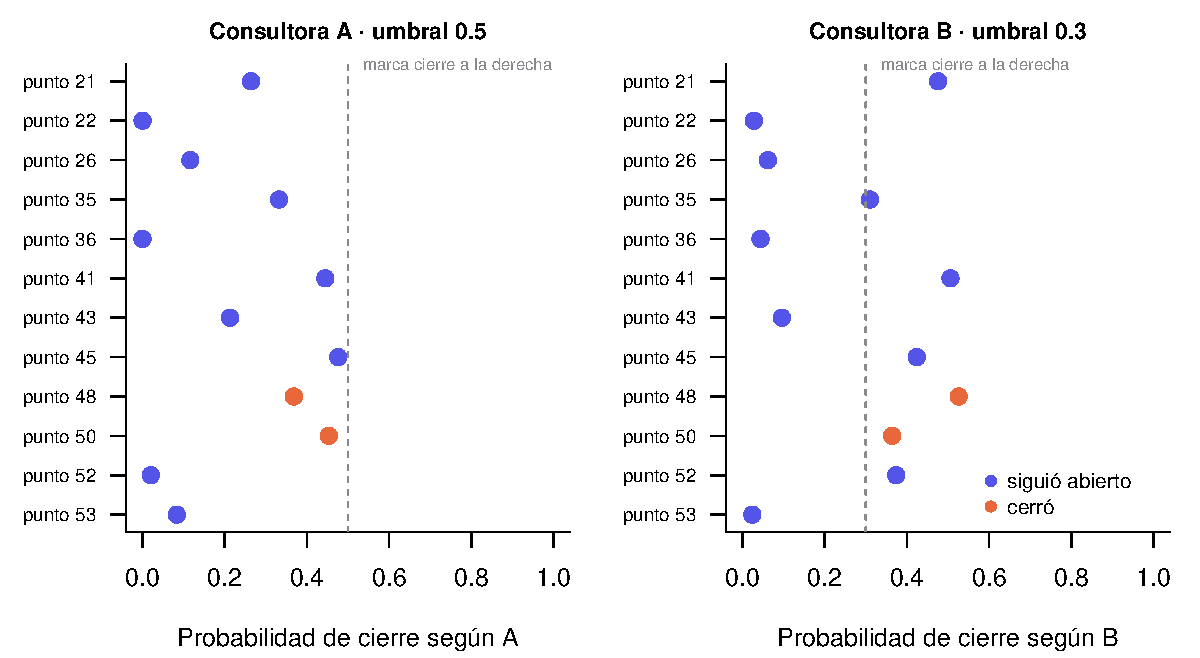
\includegraphics[width=\textwidth,height=0.62\textheight,keepaspectratio]{figures/doce_puntos.pdf}
\end{center}
\footnotesize A no marcó ninguno de los doce y se le escaparon los dos que cerraron (48 y 50). B marcó siete: atrapó los dos cierres y dio cinco falsas alarmas. Los cortes de 0.5 y 0.3 los eligieron las consultoras, no Latitud.
\end{frame}

\begin{frame}{¿Qué errores comete cada una? Los 120 del lote}
\begin{center}
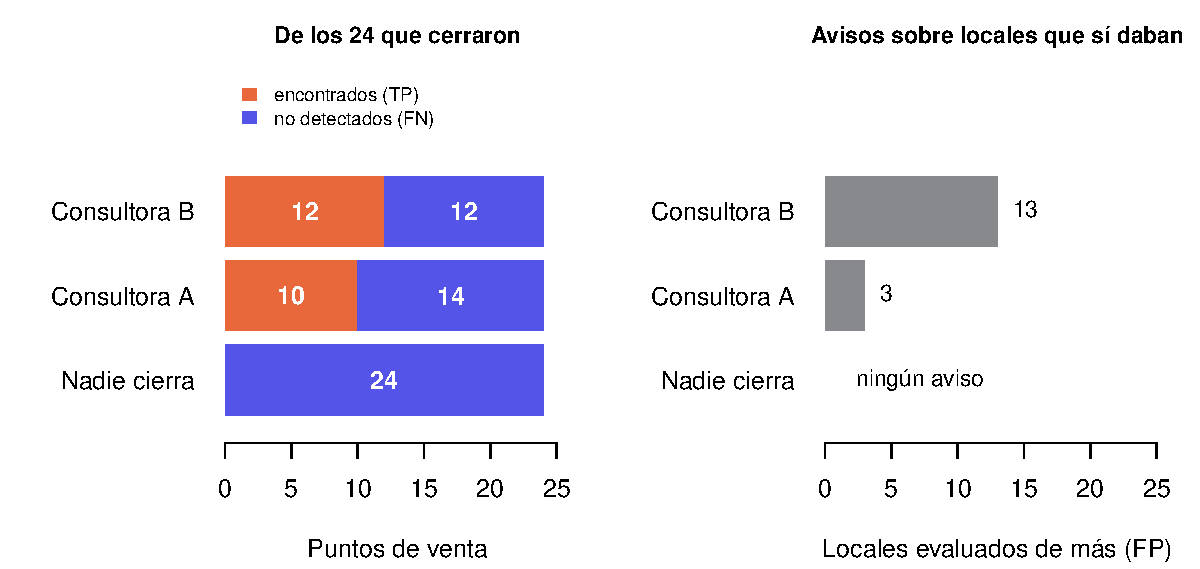
\includegraphics[width=\textwidth,height=0.6\textheight,keepaspectratio]{figures/errores_tipos.pdf}
\end{center}
\footnotesize ``Nadie cierra'' no da avisos y se le escapan los 24. A da 13 avisos: 10 acertados, 3 falsas alarmas, 14 cierres no detectados. B da 25: 12 acertados, 13 falsas alarmas, 12 no detectados.
\end{frame}

\begin{frame}{Tres métricas, tres preguntas}
\begin{columns}[T]
\begin{column}{0.58\textwidth}
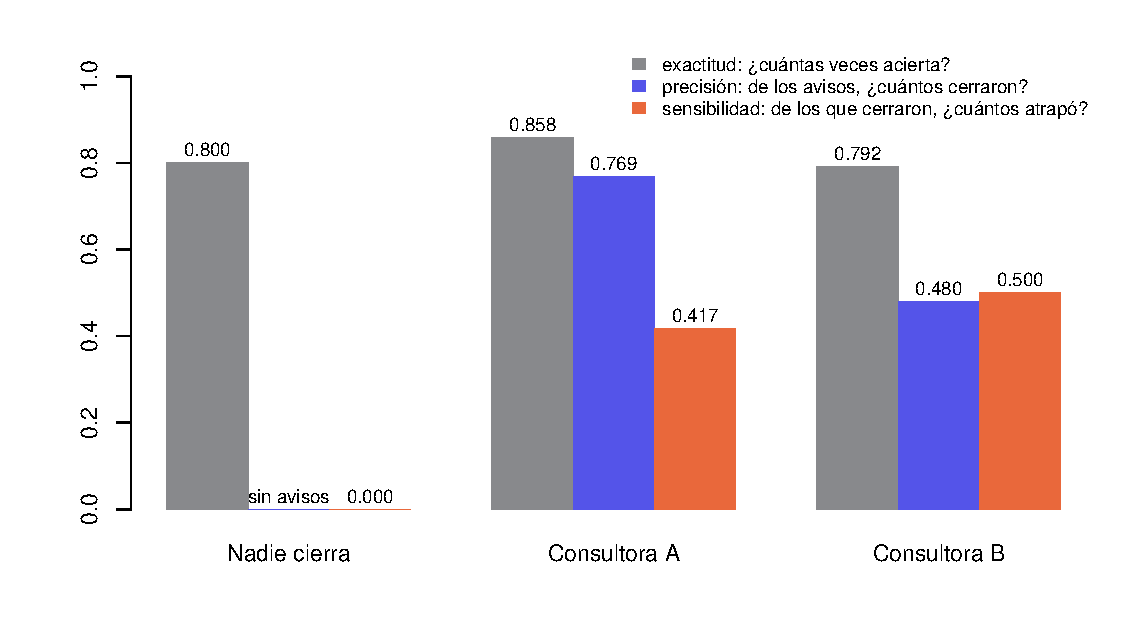
\includegraphics[width=\textwidth]{figures/metricas.pdf}
\end{column}
\begin{column}{0.42\textwidth}
\footnotesize
\begin{itemize}\itemsep5pt
  \item \textbf{Exactitud:} ¿cuántas veces acierta? Gana A (0.858). ``Nadie cierra'' saca 0.800 sin encontrar nada; B (0.792) queda por debajo.
  \item \textbf{Precisión:} de los avisos, ¿cuántos cerraron? Gana A: 0.769. B: 0.480.
  \item \textbf{Sensibilidad:} de los 24 que cerraron, ¿cuántos atrapó? Gana B: 0.500. A: 0.417. Nadie: 0.
\end{itemize}
\end{column}
\end{columns}
\medskip
\importa{Cada métrica premia a una consultora distinta. Antes de elegir hay que decidir qué pregunta le importa a Latitud, y eso lo deciden los costos.}
\end{frame}

\begin{frame}{La matriz leída en pesos}
\parada{encuesta}{¿Cuál error es más caro para Latitud: una falsa alarma o un cierre no detectado?}
\medskip
\footnotesize
\setlength{\tabcolsep}{4pt}
\begin{tabular}{@{}L{0.17\textwidth} L{0.36\textwidth} L{0.36\textwidth}@{}}
\toprule
 & \textbf{El modelo dijo ``riesgoso''} & \textbf{El modelo dijo ``viable''} \\
\midrule
\textbf{El punto de venta cerró} & \textbf{Aviso acertado (TP).} Se evalúa a fondo (12) y, con efectividad $u$, se evita una apertura fallida (250) & \textbf{Cierre no detectado (FN).} Se abre un punto de venta que cierra: 250 millones perdidos \\
\textbf{Siguió abierto} & \textbf{Falsa alarma (FP).} Se evalúa a fondo un local que sí daba: 12. Descartarlo a ciegas costaría 90 de utilidad & \textbf{Viable confirmado (TN).} Sin costo \\
\bottomrule
\end{tabular}
\medskip

\small Un cierre no detectado cuesta unas veinte veces lo que una falsa alarma. Por eso Latitud evalúa en lugar de descartar: los 12 millones son el seguro contra los 90.
\end{frame}

\begin{frame}{¿Cómo se calcula el costo de cada lista?}
\small Con las casillas del lote y 12 millones por evaluación, en cuatro pasos:

\medskip
\begin{center}
\footnotesize
\setlength{\tabcolsep}{3pt}
\renewcommand{\arraystretch}{1.15}
\begin{tabular}{@{}L{3cm} >{\centering\arraybackslash}p{1.9cm} >{\centering\arraybackslash}p{2.4cm} >{\centering\arraybackslash}p{2.4cm}@{}}
\toprule
\textbf{Paso} & \textbf{Nadie cierra} & \textbf{Consultora A} & \textbf{Consultora B} \\
\midrule
\textbf{1. Evaluaciones} (TP $+$ FP) & $0 + 0 = $ \textbf{0} & $10 + 3 = $ \textbf{13} & $12 + 13 = $ \textbf{25} \\
\textbf{2. Costo de la lista} (evaluaciones $\times$ 12) & \textbf{0} & $13 \times 12 = $ \textbf{156} & $25 \times 12 = $ \textbf{300} \\
\textbf{3. Cierres encontrados} (TP) & \textbf{0} & \textbf{10} & \textbf{12} \\
\textbf{4. Por cierre encontrado} (costo $\div$ encontrados) & no aplica & $156 \div 10 = $ \textbf{15.6} & $300 \div 12 = $ \textbf{25.0} \\
\bottomrule
\end{tabular}
\end{center}

\importa{Cada aviso cuesta lo mismo, acierte o no: cada cierre encontrado cuesta $12 \div$ precisión. A: $12 \div 0.769 = 15.6$; B: $12 \div 0.480 = 25.0$.}
\end{frame}

\begin{frame}{¿Cuánto cuesta encontrar un cierre más?}
\begin{columns}[T]
\begin{column}{0.56\textwidth}
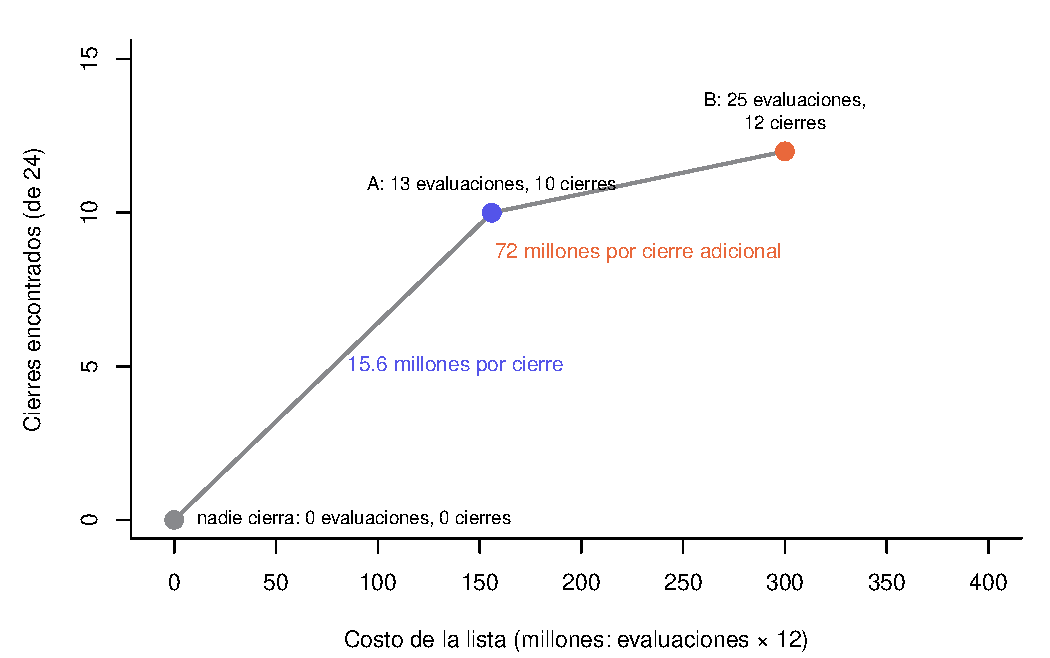
\includegraphics[width=\textwidth,height=0.52\textheight,keepaspectratio]{figures/frontera.pdf}
\end{column}
\begin{column}{0.44\textwidth}
\footnotesize
\begin{itemize}\itemsep6pt
  \item De no hacer nada a la lista de A: \textbf{15.6 millones} por cierre encontrado (10 cierres por 156).
  \item De A a B: 12 evaluaciones más (144 millones) por 2 cierres más: \textbf{72 millones por cierre adicional}.
\end{itemize}
\end{column}
\end{columns}
\importa{Ampliar la lista conviene mientras cada cierre adicional valga más de lo que cuesta encontrarlo. ¿Y cuánto vale un cierre encontrado? Depende de cuántas aperturas fallidas evita de verdad.}
\end{frame}

\begin{frame}{El beneficio neto frente a no hacer nada}
\footnotesize Encontrar un cierre no es evitarlo: el aviso dispara una evaluación, y la evaluación evita la apertura fallida solo una fracción $u$ de las veces. Beneficio neto $=$ cierres encontrados $\times\, u \times 250 -$ evaluaciones $\times\, 12$; nadie $= 0$.

\begin{center}
\scriptsize
\setlength{\tabcolsep}{3pt}
\renewcommand{\arraystretch}{1.1}
\begin{tabular}{@{}L{2.3cm} >{\centering\arraybackslash}p{1.4cm} >{\centering\arraybackslash}p{2.6cm} >{\centering\arraybackslash}p{2.6cm} >{\centering\arraybackslash}p{0.9cm}@{}}
\toprule
\textbf{Efectividad del aviso} & \textbf{Cada cierre vale} & \textbf{Consultora A} & \textbf{Consultora B} & \textbf{Gana} \\
\midrule
$u = 0.5$: evita 1 de cada 2 & 125 & $10 \times 125 - 156 = $ \textbf{1094} & $12 \times 125 - 300 = $ \textbf{1200} & B \\
$u = 0.25$: evita 1 de cada 4 & 62.5 & $10 \times 62.5 - 156 = $ \textbf{469} & $12 \times 62.5 - 300 = $ \textbf{450} & A \\
\bottomrule
\end{tabular}
\end{center}
\pause
\importa{Los modelos no cambiaron; cambió cuánto vale cada acierto. Con el supuesto base pagan los dos tramos (hasta los 72 por cierre adicional); con el pesimista, solo el primero. Las dos le ganan a no hacer nada, con holgura.}
\end{frame}

\begin{frame}{La efectividad de quiebre}
\begin{columns}[T]
\begin{column}{0.56\textwidth}
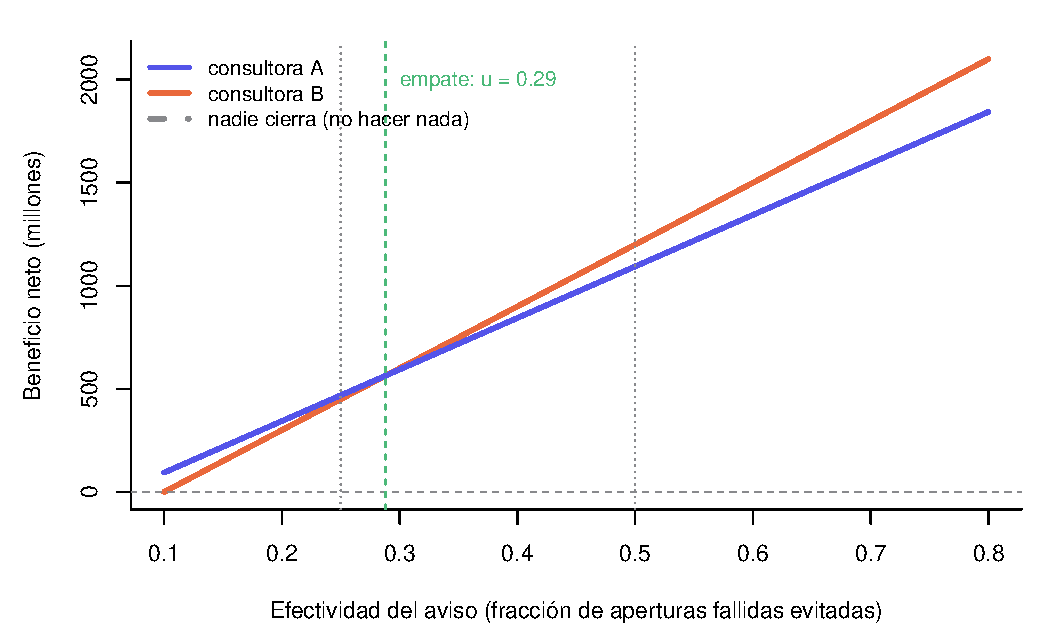
\includegraphics[width=\textwidth,height=0.45\textheight,keepaspectratio]{figures/juez_beneficio.pdf}
\end{column}
\begin{column}{0.44\textwidth}
\footnotesize
\begin{itemize}\itemsep3pt
  \item A y B empatan en $u = 12 \times 12 \div (250 \times 2) = $ \textbf{0.288}. Por debajo gana A; por encima, B.
  \item En la otra moneda: con $u = 0.5$ empatan cuando la pérdida evitada vale \textbf{144}; con $V$ por debajo gana A, por encima B.
  \item Para que valga la pena contratar: $V$ por encima de 31.2 (A) o de 50.0 (B). Latitud está lejos de ese piso.
\end{itemize}
\end{column}
\end{columns}
\importa{La elección entre A y B no la decide la exactitud: la decide un supuesto que nadie ha medido, cuántas aperturas fallidas evita de verdad una evaluación a fondo. Esa es la cifra que el task pide reportar.}
\end{frame}

\begin{frame}{El umbral también es una decisión}
\begin{columns}[T]
\begin{column}{0.58\textwidth}
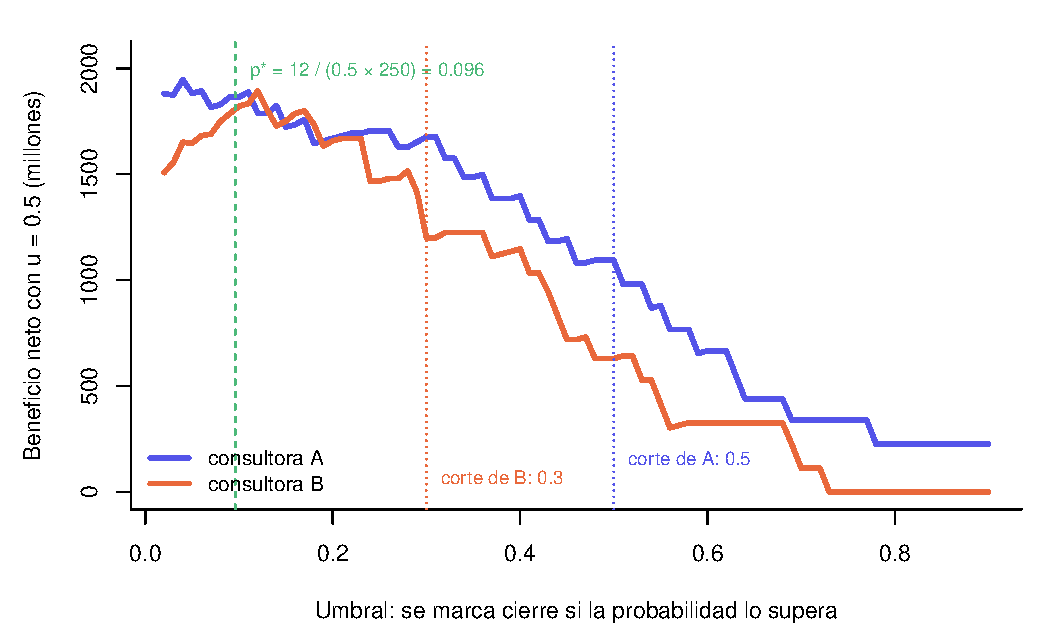
\includegraphics[width=\textwidth]{figures/umbral_beneficio.pdf}
\end{column}
\begin{column}{0.42\textwidth}
\footnotesize
\begin{itemize}\itemsep5pt
  \item Vale la pena evaluar cuando $p \times u \times V \geq c$: $p^* = c \div (u \times V) = 12 \div (0.5 \times 250) = $ \textbf{0.096}; con $u = 0.25$, \textbf{0.192}.
  \item Los cortes de 0.5 y 0.3 los eligieron las consultoras. Con $p^*$ las dos darían muchos más avisos y atraparían casi todos los cierres.
  \item \textbf{Con cupo}, el umbral no manda: si solo se pueden evaluar tres locales, se ordena por riesgo y se toman los tres primeros. Lo que importa es que el modelo ordene bien.
\end{itemize}
\end{column}
\end{columns}
\end{frame}

\begin{frame}{Las ventas: el error en pesos}
\begin{columns}[T]
\begin{column}{0.6\textwidth}
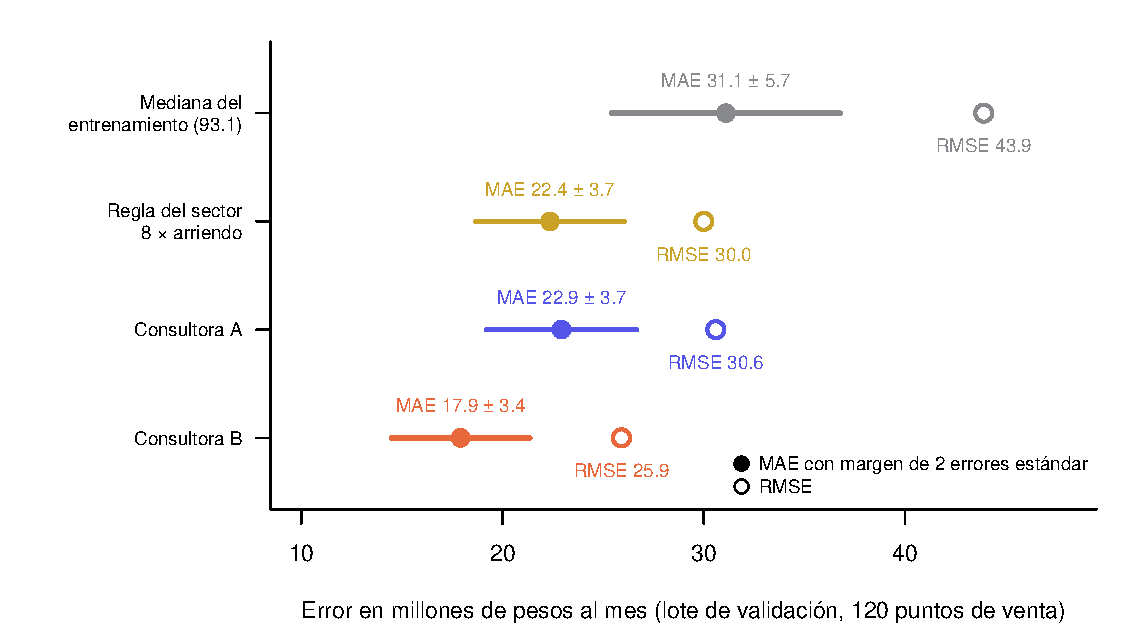
\includegraphics[width=\textwidth,height=0.5\textheight,keepaspectratio]{figures/ventas_mae.pdf}
\end{column}
\begin{column}{0.4\textwidth}
\footnotesize
\begin{itemize}\itemsep3pt
  \item \textbf{MAE:} el error promedio, en millones al mes. \textbf{RMSE:} castiga los errores grandes; la brecha delata fallas ocasionales.
  \item Regla 8 $\times$ arriendo: 22.4. A: 22.9. B: 17.9. Mediana (93.1): 31.1.
  \item Cada millón mensual mueve el VPN a cinco años en 9 millones: el MAE de B son \textbf{161 millones} de VPN por local.
\end{itemize}
\end{column}
\end{columns}
\importa{Con 120 puntos de venta, cada MAE trae un margen de dos errores estándar. Una diferencia menor que el margen no es una diferencia.}
\end{frame}

\begin{frame}{¿Le gana a la regla por más que el ruido?}
\begin{center}
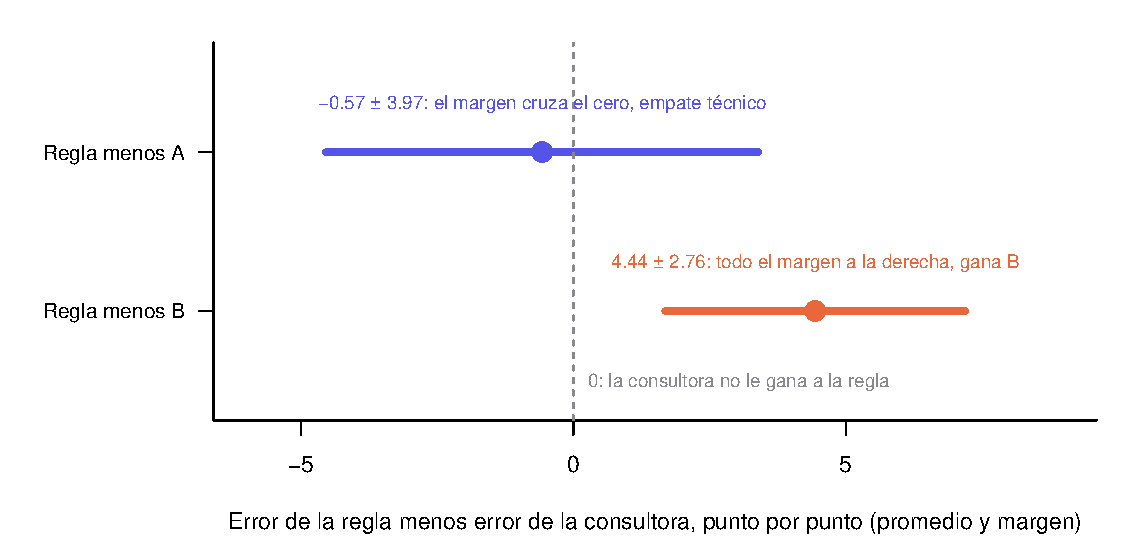
\includegraphics[width=0.78\textwidth]{figures/pareada.pdf}
\end{center}
\footnotesize
\begin{itemize}\itemsep2pt
  \item \textbf{Pareada:} punto por punto, error de la regla menos error de la consultora; se promedia y se mira el margen. El ruido común se cancela.
  \item \textbf{Regla menos A: $-0.57 \pm 3.97$.} El margen cruza el cero: \textbf{empate técnico}. Latitud ya tenía esa información gratis.
  \item \textbf{Regla menos B: $4.44 \pm 2.76$.} Todo el margen a la derecha: B le gana a la regla por unos 4.4 millones al mes por punto de venta.
\end{itemize}
\end{frame}

\begin{frame}{El giro: una nueva hoja de costos}
\parada{el giro}{Llega una cotización nueva: evaluar un local a fondo cuesta \textbf{el triple}, 36 millones en lugar de 12. La pérdida evitada sigue en 250. ¿Se sostiene la elección de B con $u = 0.5$? ¿Y la de A con $u = 0.25$? Dos minutos con la caja de costos o con la celda de R.}
\pause
\medskip
\footnotesize
% Cifras del giro: las imprime week-04/input/_datos_y_figuras_week04.R (no están en el sobre).
\begin{itemize}\itemsep3pt
  \item Con $u = 0.5$: A $= 10 \times 125 - 13 \times 36 = 782$; B $= 12 \times 125 - 25 \times 36 = 600$. \textbf{Gana A:} el segundo tramo ya no paga.
  \item Con $u = 0.25$: A $= 157$; B $= -150$. \textbf{B pierde dinero frente a no hacer nada.}
  \item La efectividad de quiebre sube de 0.288 a \textbf{0.864}: B solo gana si la evaluación evita casi nueve de cada diez aperturas fallidas.
\end{itemize}
\medskip
\importa{Las predicciones no cambiaron. Cambió lo que cuesta actuar sobre ellas, y con eso cambió la consultora. Un juicio sin hoja de costos no es un juicio.}
\end{frame}

\begin{frame}{Lo que importa}
\importa{%
\begin{enumerate}\itemsep5pt
  \item \textbf{Solo cuenta lo que el modelo no vio, y contra una vara.} El lote de validación y la regla vigente. ``Nadie cierra'' saca 80\,\% sin información; ``8 $\times$ arriendo'' empata con una consultora.
  \item \textbf{La matriz se lee en pesos.} Una falsa alarma cuesta una evaluación; un cierre no detectado, una apertura fallida. Cada acierto vale lo que evita: encontrados $\times\, u \times V$, menos evaluaciones $\times\, c$.
  \item \textbf{Una diferencia menor que el margen no es una diferencia,} y no adoptar ninguno es una respuesta: va con el costo o la efectividad que la voltearía.
\end{enumerate}}
\end{frame}

\seccion{El task y el cierre}
%% ====================================================== 3. PUENTE (65–70)
\begin{frame}{Task 4: ¿a cuál consultora le creemos?}
\begin{columns}[T]
\begin{column}{0.55\textwidth}
\textbf{Qué se entrega} (una página, en equipo, antes de la sesión 5):
\begin{itemize}\itemsep2pt
  \item las dos tablas del líder, cierre y ventas, con el margen, el costo marginal de A a B y la efectividad de quiebre (2.0, contra el sobre);
  \item la recomendación por target: A, B o ninguna, justificada al elegir \textbf{y al descartar}, en las palabras del negocio (1.5);
  \item la sensibilidad: qué efectividad y qué pérdida evitada voltean la decisión, y de qué lado está el supuesto defendible (1.0);
  \item el acta y la declaración (0.5).
\end{itemize}
\end{column}
\begin{column}{0.45\textwidth}
\begin{exampleblock}{En el cierre de la sesión 5}
Dos equipos al azar dicen a quién eligieron y por qué descartaron a las otras. El giro como pregunta: si evaluar costara el triple, ¿se sostiene? Y qué hace Latitud con un empate técnico.
\end{exampleblock}
\small En el memo no hay TP ni FP: hay aperturas fallidas evitadas y locales buenos descartados.
\end{column}
\end{columns}
\end{frame}

%% ====================================================== 4. CIERRE (70–90)
\begin{frame}{Cierre: la cacería del task 3}
\begin{enumerate}\itemsep8pt
  \item \textbf{Las cifras contra el sobre} (6 minutos). Dos equipos al azar, dos minutos cada uno, expositor al azar: un hallazgo con su cifra. Se abre el sobre de la semana 3 y se compara. Si no coincide, ¿de dónde venía la diferencia?
  \item \textbf{¿Quién atrapó la fuga?} (6 minutos). La columna prohibida: cuántos equipos la excluyeron antes de modelar y con qué regla (el momento de la decisión). Qué habría pasado con un modelo que la usara.
  \item \textbf{¿Qué hizo el agente de más?} (5 minutos). Un hallazgo que el agente propuso y el equipo descartó; una cifra que el agente dio y el equipo no pudo reproducir.
  \item \textbf{Dudas} (3 minutos): el task 4, la caja de costos y las celdas de la tabla del líder.
\end{enumerate}
\end{frame}

\begin{frame}{Referencias}
\small
\begin{itemize}\itemsep4pt
  \item Kleinberg, J., Lakkaraju, H., Leskovec, J., Ludwig, J. y Mullainathan, S. (2018). Human decisions and machine predictions. \emph{Quarterly Journal of Economics}, 133(1), 237--293.
  \item Kleinberg, J., Ludwig, J., Mullainathan, S. y Obermeyer, Z. (2015). Prediction policy problems. \emph{American Economic Review: Papers \& Proceedings}, 105(5), 491--495.
  \item Sosa Escudero, W. (2019). \emph{Big data}. Siglo XXI. El capítulo sobre los límites del análisis de datos.
  \item Latitud S.A.S., gerencia de expansión (2026). \emph{Estudio de aperturas: 480 puntos de venta de conveniencia}. \texttt{predicciones\_consultoras.csv}, \texttt{costos\_decision.csv} y el sobre de la semana 4.
\end{itemize}
\end{frame}

\end{document}
